\documentclass[11pt]{article}
\usepackage{amssymb}
\usepackage{amsthm}
\usepackage{enumitem}
\usepackage{amsmath}
\usepackage{bm}
\usepackage{adjustbox}
\usepackage{mathrsfs}
\usepackage{graphicx}
\usepackage{siunitx}
\usepackage[mathscr]{euscript}

\title{\textbf{Solved selected problems of Classical Mechanics - Taylor}}
\author{Franco Zacco}
\date{}

\addtolength{\topmargin}{-3cm}
\addtolength{\textheight}{3cm}

\newcommand{\hatr}{\bm{\hat{r}}}
\newcommand{\hatx}{\bm{\hat{x}}}
\newcommand{\haty}{\bm{\hat{y}}}
\newcommand{\hatz}{\bm{\hat{z}}}
\newcommand{\hatth}{\bm{\hat{\theta}}}
\newcommand{\hatphi}{\bm{\hat{\phi}}}
\newcommand{\hatrho}{\bm{\hat{\rho}}}
\theoremstyle{definition}
\newtheorem*{solution*}{Solution}

\begin{document}
\maketitle
\thispagestyle{empty}

\section*{Chapter 2 - Projectiles and Charged Particles}

	\begin{proof}{\textbf{2.1}}
        The equation for this baseball is
        $$\frac{f_{quad}}{f_{lin}} = 1.6 \times 10^3 \cdot 0.07 \cdot v$$
        to find the speed at which the two forces are important we need to find
        a value for $v$ such that $f_{quad}/f_{lin} = 1$ then
        $$v = \frac{1}{1.6 \times 10^3 \cdot 0.07} = 0.0089~m/s$$
        In this case the velocity is so small that even though both forces are
        equally important, they could be neglected.\\
        For velocities bigger than $0.0089~m/s$, $f_{quad}$ term start having
        more impact than the linear term so we could treat the drag force as
        purely quadratic.\\\\
        For a beach ball of diameter $70~cm$ we have that
        $$\frac{f_{quad}}{f_{lin}} = 1.6 \times 10^3 \cdot 0.7 \cdot v$$
        then the $v$ such that $f_{quad}/f_{lin} = 1$ we have that
        $$v = \frac{1}{1.6 \times 10^3 \cdot 0.7} = 0.00089~m/s$$

    \end{proof}
	\begin{proof}{\textbf{2.2}}
        The equation according Stoke's law is given by
        $$f_{lin} = 3 \pi \eta D v$$
        if we take $\beta = 3 \pi \eta$ then $b = \beta D$ we have that
        $$f_{lin} = bv$$
        which has the form we wanted.\\
        On the other hand, if we take $\eta = 1.7 \times 10^{-5}~si{Ns/m^2}$ then
        $$\beta = 1.6 \times 10^{-4}~\si{Ns/m^2}$$
        which is the given value for $\beta$.
    \end{proof}
	\begin{proof}{\textbf{2.3}}
        \begin{itemize}
            \item [(a)] Given that the drag force equations for a sphere are
            $$f_{lin} = 3 \pi \eta D v \quad\quad f_{quad} = \kappa \varrho A v^2$$
            then if $A = \pi (D/2)^2$ we have that
            \begin{align*}
                \frac{f_{quad}}{f_{lin}} &= \frac{\kappa \varrho A v^2}{3 \pi \eta D v}\\
                    &= \frac{\kappa \varrho \pi (D/2)^2 v^2}{3 \pi \eta D v}\\
                    &= \frac{\kappa \varrho D v}{12 \eta}
            \end{align*}
            knowing that $R = Dv\varrho / \eta$ and $\kappa = 1/4$ for a sphere
            then
            $$\frac{f_{quad}}{f_{lin}} = \frac{R}{4 \cdot 12} = \frac{R}{48}$$

            \item [(b)] Given a steel ball bearing of diameter
            $D = 2 \si{mm} = 0.002 \si{m}$ moving at $v = 5 \si{cm/s} = 0.05 \si{m/s}$
            with density $\varrho = 1.3 \si{g/cm^3} = 1300 \si{kg/m^3}$ and
            viscosity $\eta = 12 \si{Ns/m^2}$ then replacing the values in the
            Reynolds number equation we get that
            $$R = 0.01083$$
        \end{itemize}
    \end{proof}
	\begin{proof}{\textbf{2.6}}
        \begin{itemize}
            \item[(a)] The equation $v_y = v_{ter}(1 - e^{-t/\tau})$ corresponds
            to the velocity of an object dropped from rest where $v_{ter} = mg/b$
            and $\tau = m/b$, if we use the first two terms in the Taylor series
            for $e^x = 1 + x + x^2/2! + ...$ and we replace that in the equation
            for the velocity of an object dropped from rest we get that
            \begin{align*}
                v_y &= v_{ter}(1 - e^{-t/\tau}) \\
                    &= v_{ter}(1 - (1 + (-t/\tau)))\\
                    &= \frac{mg}{b}(1 - 1 + t/\tau)\\
                    &= \frac{mg}{b}\left(\frac{tb}{m}\right)\\
                    &= gt
            \end{align*}
            then we notice that if $t$ is small the approximation with two terms
            of the series gives us a correct answer for the velocity since we
            expect that the velocity has a neglectable value for the air
            resistance at that moment.
            \item[(b)] In the same way the equation
            $y(t) = v_{ter}t + (v_{y0} - v_{ter})\tau(1 - e^{-t/\tau})$
            represents the position for a dropped object, if we replace the
            first three terms of the Taylor series for $e^x$ in the equation
            and we consider that $v_{y0} = 0$ we have that
            \begin{align*}
                y(t) &= v_{ter}t + (0 - v_{ter})\tau(1 - e^{-t/\tau})\\
                     &= v_{ter}t - v_{ter}\tau(1 - (1 + (-t/\tau) + \frac{(-t/\tau)^2}{2!}))\\
                     &= v_{ter}t - v_{ter}\tau(t/\tau - \frac{(-t/\tau)^2}{2})\\
                     &= v_{ter}t - v_{ter}t + \frac{1}{2}\frac{v_{ter}}{\tau}t^2\\
                     &= \frac{1}{2}\frac{mg}{b}\frac{1}{m/b}t^2\\
                     &= \frac{1}{2}gt^2
            \end{align*}
            then this is the position for an object falling in the vacuum where
            air resistance is neglected, which is the case for the first moments
            of the object dropped where the air resistance can be neglected.
        \end{itemize}
    \end{proof}
	\begin{proof}{\textbf{2.9}}
        We are requested to integrate the equation
        $$\frac{m~dv_y}{v_y - v_{ter}} = -b~dt$$
        so we integrate the equation both sides from $0$ to $t$ on the
        right hand side and on the left hand side the integration should be
        from $v_{y0}$ to $v_{y}$, to avoid confusion with the integration
        limit we renamed the variable on the left hand side of the equation to
        $v_{y}'$.        
        \begin{align*}
            \int_{v_{y0}}^{v_y} \frac{m~dv_y'}{v_y' - v_{ter}} &= \int_0^t -b~dt \\
            m \int_{v_{y0}}^{v_y} \frac{dv_y'}{v_y' - v_{ter}} &= -b \int_0^t dt \\
            m[\log(v_y - v_{ter}) - \log(v_{y0} - v_{ter})] &= -b[t - 0]\\
            \log(\frac{v_y - v_{ter}}{v_{y0} - v_{ter}}) &= \frac{-b}{m}t\\
            \frac{v_y - v_{ter}}{v_{y0} - v_{ter}} &= e^{-t/\tau}\\
            v_y &= v_{ter} + (v_{y0} - v_{ter})e^{-t/\tau}
        \end{align*}
        Notice that $\tau = m/b$. Therefore we got the same result as with the
        inspection method.
    \end{proof}
\cleardoublepage
	\begin{proof}{\textbf{2.11}}
        \begin{itemize}
        \item[(a)] In this case since the y-axis is looking upwards we have the
        following equation of motion
        $$m\dot{v_y} = -bv_y - mg$$
        where both the linear drag force and the gravity point downward. From
        now on we consider $v_y = v$ so we can also write this equation as
        $$m\dot{v} = -b(v + v_{ter})$$
        with $v_{ter} = mg/b$, and we know the solution for this kind of
        equations, so we get that
        $$v(t) = (v_{0} + v_{ter})e^{-t/\tau} - v_{ter}$$
        Now integrating this equation, from $0$ to $t$ we get $y(t)$ as
        \begin{align*}
            y(t) &= \int_0^tv(t')~dt'\\
                 &= \int_0^t [(v_{0} + v_{ter})e^{-t'/\tau} - v_{ter}]~dt'\\
                 &= (v_{0} + v_{ter})\tau (1 - e^{-t/\tau}) - v_{ter}t
        \end{align*}
        \item[(b)] To find the moment at which the object reaches the highest
        point we need to find where the derivative of the position's equation
        is zero so, we first derivate $y(t)$ as
        $$\frac{dy(t)}{dt} = (v_0 + v_{ter})e^{-t/\tau} - v_{ter}$$
        then making the equation equal to 0 we find the time $t$ at which the
        position of the object reaches its highest point
        \begin{align*}
            (v_0 + v_{ter})e^{-t/\tau} - v_{ter} &= 0 \\
            e^{-t/\tau} &= \frac{v_{ter}}{v_0 + v_{ter}} \\
            -t/\tau &= \log\left(\frac{v_{ter}}{v_0 + v_{ter}}\right) \\
             t &= -\tau [\log(v_{ter}) - \log(v_0 + v_{ter})] \\
             t &= \tau [\log(v_0 + v_{ter}) - \log(v_{ter})] \\
             t &= \tau \log\left(\frac{v_0}{v_{ter}} + 1\right)
        \end{align*}
        now replacing this value in the equation for $y(t)$ we get that
        \begin{align*}
            y_{max} &= (v_{0} + v_{ter})\tau (1 - e^{-\log(1 + \frac{v_0}{v_{ter}})}) - v_{ter}\tau \log\left(1 + \frac{v_0}{v_{ter}}\right)\\
                &= (v_{0} + v_{ter})\tau(1 - \frac{v_{ter}}{v_0 + v_{ter}}) - v_{ter}\tau \log\left(1 + \frac{v_0}{v_{ter}}\right)\\
                &= (v_{0} + v_{ter})\tau - v_{ter}\tau - v_{ter}\tau \log\left(1 + \frac{v_0}{v_{ter}}\right)\\
                &= v_{0}\tau - v_{ter}\tau \log\left(1 + \frac{v_0}{v_{ter}}\right)\\
                &= \tau\left[v_{0} - v_{ter} \log\left(1 + \frac{v_0}{v_{ter}}\right)\right]\\
        \end{align*}
        \item[(c)] Given that if the drag force is very small, the terminal
        velocity is very big and therefore $v_0/v_{ter}$ is very small, then we
        can approximate $\log(1 + v_0/v_{ter})$ by two terms of its Taylor series
        which give us
        \begin{align*}
            y_{max} &= \tau\left[v_{0} - v_{ter}\left(
                \frac{v_0}{v_{ter}} -
                \frac{1}{2}\left(\frac{v_0}{v_{ter}}\right)^2
                \right)
            \right]\\
                    &= \tau\left[
                        v_{0} -
                        v_0 +
                        \frac{1}{2} \frac{v_0^2}{v_{ter}}
                    \right]\\
                    &= \tau \frac{1}{2} \frac{v_0^2}{v_{ter}}\\
                    &= \frac{1}{2} \frac{m}{b} \frac{v_0^2}{\frac{mg}{b}}\\
                    &= \frac{1}{2}\frac{v_0^2}{g}
        \end{align*}
        therefore $y_{max}$ is reduced to it's vacuum value.
        \end{itemize} 
    \end{proof}
\cleardoublepage
	\begin{proof}{\textbf{2.17}}
        From the equation for $x(t)$ we want to get $t$ as a function of $x$
        then
        \begin{align*}
            x &= v_{x0}\tau(1 - e^{-t/\tau})\\
            \frac{x}{v_{x0}\tau} &= 1 - e^{-t/\tau}\\
            1 - \frac{x}{v_{x0}\tau} &= e^{-t/\tau}\\
            \log(1 - \frac{x}{v_{x0}\tau}) &= -t/\tau\\
            -\tau \log(1 - \frac{x}{v_{x0}\tau}) &= t
        \end{align*}
        now we replace the equation for $t$ in the equation of $y(t)$ to get
        $y$ as a function of $x$
        \begin{align*}
            y(t) &= (v_{y0} + v_{ter})\tau(1 - e^{-t/\tau}) - v_{ter}t\\
                 &= (v_{y0} + v_{ter})\tau(1 - e^{\log(1 - \frac{x}{v_{x0}\tau})})
                 + v_{ter}\tau \log(1 - \frac{x}{v_{x0}\tau})\\
                 &= (v_{y0} + v_{ter})\tau(1 - (1 - \frac{x}{v_{x0}\tau}))
                 + v_{ter}\tau \log(1 - \frac{x}{v_{x0}\tau})\\
                 &= (v_{y0} + v_{ter})\tau\frac{x}{v_{x0}\tau}
                 + v_{ter}\tau \log(1 - \frac{x}{v_{x0}\tau})\\
                 &= \frac{v_{y0} + v_{ter}}{v_{x0}}x
                 + v_{ter}\tau \log(1 - \frac{x}{v_{x0}\tau})
        \end{align*}
        which is the equation we wanted. 
    \end{proof}
	\begin{proof}{\textbf{2.19}}
        \begin{itemize}
            \item[(a)] We know that the equations for a motion where no air
            resistance is considered are
            \begin{align}
                x &= v_{x0}t + x_0\\
                y &= y_0 + v_{y0}t - \frac{1}{2}gt^2
            \end{align}
            considering $x_0 = y_0 = 0$ and from (1) we write $t$ in terms of
            $x$ we get that
            $$t = \frac{x}{v_{x0}}$$
            then we replace this value of $t$ in (2) to get
            $$y = \frac{v_{y0}}{v_{x0}}x - \frac{1}{2}g\left(\frac{x}{v_{x0}}\right)^2$$
            \item[(b)] Given that $\tau$ and $v_{ter}$ approach infinity we can
            approximate\\
            $\log(1 - x/v_{x0}\tau)$ by its Taylor series as
            $$\log(1 - \frac{x}{v_{x0}\tau}) = -\frac{x}{v_{x0}\tau} - \frac{1}{2}\frac{x^2}{v_{x0}^2\tau^2}$$
            then the equation for $y$ in terms of $x$ is given by
            \begin{align*}
                y &= \frac{v_{y0} + v_{ter}}{v_{x0}}x + v_{ter}\tau\left[-\frac{x}{v_{x0}\tau} - \frac{1}{2}\frac{x^2}{v_{x0}^2\tau^2}\right]\\
                  &= \frac{v_{y0}}{v_{x0}}x + \frac{v_{ter}}{v_{x0}}x -
                  \frac{v_{ter}}{v_{x0}}x - \frac{1}{2}\frac{v_{ter}x^2}{v_{x0}^2\tau}\\
                  &= \frac{v_{y0}}{v_{x0}}x - \frac{1}{2}g\left(\frac{x}{v_{x0}}\right)^2
            \end{align*}
            where we used that $v_{ter}/\tau = g$. Finally we get the same
            equation for a motion where no air resistance is considered.
        \end{itemize}
    \end{proof}
\cleardoublepage
    \begin{proof}{\textbf{2.20}}
        Below we show the trajectories for $t$ between 0 and 3 with different
        $v_{ter} = \tau$ which means different values for drag. We are
        assuming $v_{x0} = v_{y0} = 1$ and $g = 1$. Finally the trajectory
        shown for $v_{ter} = \infty$ is described by
        \begin{align*}
            x &= v_{x0}t + x_0\\
            y &= y_0 + v_{y0}t - \frac{1}{2}gt^2
        \end{align*}
        that was calculated in last problem.\\
        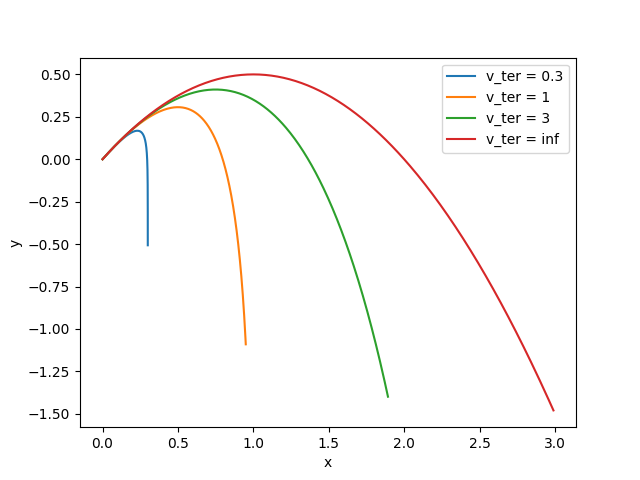
\includegraphics{taylor-2.20.png}
    \end{proof}
    \begin{proof}{\textbf{2.22}}
        \begin{itemize}
            \item [(a)] We know that for the vacuum the range equation is
            $$R_{vac} = \frac{2v_{x0}v_{y0}}{g}$$
            if we assume $g = 1$ and $v_0 = 1$ then $v_{x0} = \cos(\theta)$ and
            $v_{y0} = \sin(\theta)$ also we know that the maximum range occurs
            at $\theta = \pi / 4$ then
            $$R_{vac} = \frac{2\cos(\pi /4)\sin(\pi / 4)}{1} = 1$$
            \item [(b)] If we solve the equation for $R$ in a linear medium by
            binary search with the code shown below
            \begin{verbatim}
            def binary_search(theta=0.75):
                R_max = 0.4
                R_min = 0.6
                epsilon = 0.000001
                f_mid = 1000

                while abs(f_mid) > epsilon:
                    R_mid = R_min + ((R_max - R_min)/2)
                    f_mid = func(R_mid, theta)
                    if f_mid > 0:
                        R_max = R_mid
                    elif f_mid < 0:
                        R_min = R_mid

                return f_mid, R_mid
            \end{verbatim}
            we get that for $R = 0.4995$ the function value is less than
            the epsilon we set. Therefore the Range in a linear medium when
            $\theta = 0.75$ is $R = 0.4995$.
\cleardoublepage
            \item [(c)(d)] By doing binary search for different values of
            $\theta$ in a range between 0.1 and 0.8, we obtained the following
            plot\\
            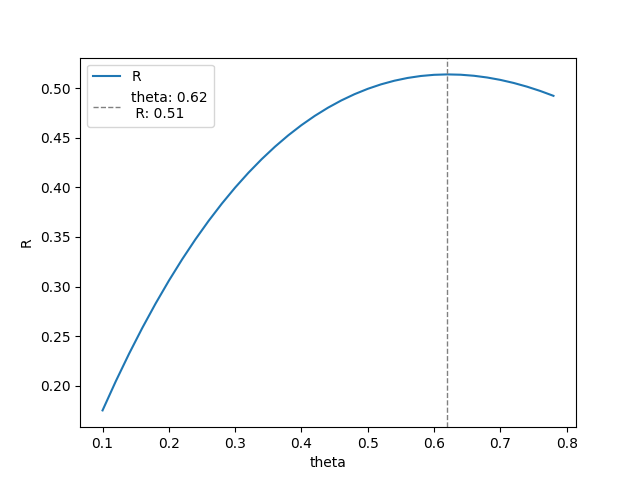
\includegraphics{taylor-2.22.png}
            It is also plotted the $\theta$ angle for which $R$ is maximum,
            which happens to be at 0.62 and we obtained an $R$ maximum of 0.51.
        \end{itemize}
    \end{proof}
    \begin{proof}{\textbf{2.24}}
        \begin{itemize}
            \item[(a)] We defined $v_{ter} = \sqrt{mg/c}$ where
            $m = 4/3 \pi (D/2)^3\varrho_{sph}$ which is the multiplication of
            the sphere volume and the density and
            $c = \kappa \varrho_{air} \pi (D/2)^2$ where $\kappa = 1/4$ with all that we get that
            \begin{align*}
                v_{ter} &= \sqrt{\frac{4/3 \pi (D/2)^3\varrho_{sph}g}{\kappa \varrho_{air} \pi (D/2)^2}}\\
                        &= \sqrt{\frac{8 D\varrho_{sph}g}{3\varrho_{air}}}\\
            \end{align*}
\cleardoublepage
            \item[(b)] Given that $v_{ter}$ is proportional to $\sqrt{\varrho_{sph}}$
            then if the sphere 1 is denser than sphere 2 we have that
            $\varrho_{sph1} > \varrho_{sph2}$ so $\sqrt{\varrho_{sph1}} > \sqrt{\varrho_{sph2}}$
            and therefore $v_{ter}$ for sphere 1 is going to be bigger than
            for sphere 2.
            \item[(c)] Also $v_{ter}$ is proportional to $\sqrt{D}$
            then if the sphere 1 is larger   than sphere 2 we have that
            $D_1 > D_2$ so $\sqrt{D_1} > \sqrt{D_2}$
            and therefore $v_{ter}$ for sphere 1 is going to be bigger than
            for sphere 2. 
        \end{itemize}
    \end{proof}
    \begin{proof}{\textbf{2.27}}
        The Newton's second law equation in this case assuming the positive
        x-axis is in the direction of the incline is given by
        $$m\frac{dv}{dt} = -mg\sin(\theta) - cv^2$$
        if we define $v_{ter} = \sqrt{mg\sin{\theta}/c}$ we have that
        \begin{align*}
            \frac{dv}{dt} &= g\sin(\theta)\left(-1 - \frac{v^2}{v_{ter}^2}\right)\\
            \int_{v_0}^v\frac{dv}{\left(-1 - \frac{v^2}{v_{ter}^2}\right)}
                &= \int_{0}^tg\sin(\theta)dt\\
            v_{ter}\left(-\arctan(\frac{v}{v_{ter}}) + \arctan(\frac{v_{0}}{v_{ter}})\right)
                &= g\sin(\theta)t\\
            -\arctan(\frac{v}{v_{ter}}) &= \frac{g\sin(\theta)t}{v_{ter}} - \arctan(\frac{v_0}{v_{ter}})\\
            v &= \tan(\arctan(\frac{v_0}{v_{ter}}) - \frac{g\sin(\theta)t}{v_{ter}})
        \end{align*}
        To find the time it takes the upward journey we need to solve $v(t)=0$
        since the velocity should be $0$ when the puck is at the top.
        \begin{align*}
            0 &= \tan(\arctan(\frac{v_0}{v_{ter}}) - \frac{g\sin(\theta)t_{top}}{v_{ter}})\\
            \frac{g\sin(\theta)t_{top}}{v_{ter}} &= \arctan(\frac{v_0}{v_{ter}}) \\
            t_{top} &= \frac{v_{ter}}{g\sin(\theta)}\arctan(\frac{v_0}{v_{ter}})
        \end{align*} 
    \end{proof}
    \begin{proof}{\textbf{2.32}}
        \begin{itemize}
            \item[(a)] If we think of the boundary case where there is no air
            resistance then the trajectory is parabolic, then the velocity must
            be it's derivative therefore a linear equation which never stops
            growing therefore never finding its $v_{ter}$.
            \item[(b)] If we write $f/mg$ for linear and quadratic drag cases
            we get that
            $$\frac{f_{lin}}{mg} = \frac{v}{v_{ter}} \quad\quad \frac{f_{quad}}{mg} = \frac{v^2}{v^2_{ter}}$$
            given that the velocity is much less than $v_{ter}$ when small
            air resistance is present, we see from the equations that for the
            quadratic equation the effect is bigger since if $v/v_{ter} < 1$
            then $v^2/v_{ter}^2 \ll 1$.
        \end{itemize}
    \end{proof}
    \begin{proof}{\textbf{2.35}}
        \begin{itemize}
            \item[(a)] From the equation of motion $m\dot{v} = mg - cv^2$ and
            defining $v_{ter} = \sqrt{\frac{mg}{c}}$ we get that
            \begin{align*}
                m\dot{v} &= mg - cv^2\\
                \dot{v} &= g\left(1 - \frac{v^2}{v_{ter}^2}\right)\\
                \int_0^v\frac{dv'}{\left(1 - \frac{v'^2}{v_{ter}^2}\right)}
                    &= \int_0^tgdt' \quad\text{(variable replacement)}\\
                v_{ter} \tanh^{-1}(\frac{v}{v_{ter}}) &= gt\\
                \frac{v}{v_{ter}} &= \tanh(\frac{gt}{v_{ter}})\\
                v &= v_{ter}\tanh(\frac{gt}{v_{ter}})
            \end{align*}
            to find the position we need to solve the following
            \begin{align*}
                \frac{dy}{dt} &= v_{ter}\tanh(\frac{gt}{v_{ter}})\\
                \int_{0}^y dy' &= \int_0^t v_{ter}\tanh(\frac{gt'}{v_{ter}})dt'
                    \quad\text{(variable replacement)}\\
                y &= \frac{v_{ter}^2}{g} \log(\cosh(\frac{gt}{v_{ter}}))
            \end{align*}
            \item[(b)] Given that $\tau = v_{ter}/g$ we can write the above
            equations as
            \begin{align*}
                v &= v_{ter} \tanh(\frac{t}{\tau}) \quad\text{and}\\
                y &= \tau v_{ter} \log(\cosh(\frac{t}{\tau}))
            \end{align*}
            if $t=\tau$ then
            $$v = v_{ter} \tanh(1) = v_{ter} 0.7615$$
            which means that the velocity reaches $76\%$ of its terminal velocity
            when $t=\tau$.\\
            For $t = 2\tau$ we have that $v = v_{ter}0.964$, which is the $96\%$
            of $v_{ter}$ and for $t = 3\tau$ we have that $v = v_{ter}0.995$
            which is the $99\%$ of $v_{ter}$.
            \item[(c)] When $t \gg \tau$ we can approximate $\cosh$ from its
            definition as \\ $\cosh(z) \approx e^z/2$ then
            \begin{align*}
                y &= \tau v_{ter} \log(\cosh(\frac{t}{\tau}))\\
                  &\approx \tau v_{ter} \log(\frac{e^\frac{t}{\tau}}{2})\\
                  &\approx \tau v_{ter} \left(\frac{t}{\tau} - \log(2)\right)\\
                  &\approx v_{ter}t - v_{ter}\tau \log(2)
            \end{align*}
            \item[(d)] When $t$ is small we can approximate the logarithm and
            the hyperbolic cosine functions by their Taylor series as
            $\log(1 + t) = t - t^2/2$ and $\cosh(x) = 1 + x^2/2!$ then
            \begin{align*}
                y &= \tau v_{ter} \log(\cosh(\frac{t}{\tau}))\\
                  &\approx \tau v_{ter} \log(1 + \frac{(t/\tau)^2}{2})\\
                  &\approx \tau v_{ter} \left(\frac{(t/\tau)^2}{2} - \frac{((t/\tau)^2/2)^2}{2}\right)\\
                  &\approx \tau v_{ter} \left(\frac{(t/\tau)^2}{2} - \frac{(t/\tau)^4}{8}\right)\\
                  &\approx \frac{v_{ter}}{\tau} \frac{t^2}{2}\\
                  &\approx g \frac{t^2}{2}
            \end{align*}
            given that $t$ is already small we removed the term $(t/\tau)^4/8$
            from the equation since its negligible.
        \end{itemize}
    \end{proof}
\cleardoublepage
    \begin{proof}{\textbf{2.38}}
        \begin{itemize}
        \item[(a)] The Newton's second law equation in this case assuming the
        positive y-axis is in an upward direction is given by
        $$m\frac{dv}{dt} = -mg - cv^2$$
        if we define $v_{ter} = \sqrt{mg/c}$ we have that
        \begin{align*}
            \frac{dv}{dt} &= g\left(-1 - \frac{v^2}{v_{ter}^2}\right)\\
            \int_{v_0}^v\frac{dv}{\left(-1 - \frac{v^2}{v_{ter}^2}\right)}
                &= \int_{0}^tgdt\\
            v_{ter}\left(-\arctan(\frac{v}{v_{ter}}) + \arctan(\frac{v_{0}}{v_{ter}})\right)
                &= gt\\
            -\arctan(\frac{v}{v_{ter}}) &= \frac{gt}{v_{ter}} - \arctan(\frac{v_0}{v_{ter}})\\
            v &= \tan\left(\arctan(\frac{v_0}{v_{ter}}) - \frac{gt}{v_{ter}}\right)
        \end{align*}
        \item[(b)] To find the time it takes the upward journey we need to solve
        $v(t)=0$ since the velocity should be $0$ when the projectile is at the
        top, then
        \begin{align*}
            0 &= \tan\left(\arctan(\frac{v_0}{v_{ter}}) - \frac{gt_{top}}{v_{ter}}\right)\\
            \frac{gt_{top}}{v_{ter}} &= \arctan(\frac{v_0}{v_{ter}}) \\
            t_{top} &= \frac{v_{ter}}{g}\arctan(\frac{v_0}{v_{ter}})
        \end{align*}
        \item[(c)] For a baseball with $v_{ter} = 35 \si{m/s}$ we have that\\
        $v_0 = 1 \si{m/s}$ then $t_{top} = 0.102 \si{s}$ and in vacuum 
        $t_{top} = 0.102\si{s}$\\
        $v_0 = 10 \si{m/s}$ then $t_{top} = 0.993 \si{s}$ and in vacuum 
        $t_{top} = 1.020\si{s}$\\
        $v_0 = 20 \si{m/s}$ then $t_{top} = 1.854 \si{s}$ and in vacuum 
        $t_{top} = 2.040\si{s}$\\
        $v_0 = 30 \si{m/s}$ then $t_{top} = 2.53 \si{s}$ and in vacuum 
        $t_{top} = 3.061\si{s}$\\
        $v_0 = 40 \si{m/s}$ then $t_{top} = 3.042 \si{s}$ and in vacuum 
        $t_{top} = 4.081\si{s}$\\
        \end{itemize}
    \end{proof}
\cleardoublepage
    \begin{proof}{\textbf{2.41}}
    The Newton's second law equation in this case assuming the
    positive y-axis is in an upward direction is given by
    $$m\dot{v} = -mg - cv^2$$
    if we define $v_{ter} = \sqrt{mg/c}$ and we take $mg$ as factor we have that
    \begin{align*}
        \dot{v} &= g\left(-1 - \frac{v^2}{v_{ter}^2}\right)\\
        \dot{v} &= -g\left(1 + \frac{v^2}{v_{ter}^2}\right)\\
        v\frac{dv}{dy} &= -g\left(1 + \frac{v^2}{v_{ter}^2}\right)\\
        \int_{v_0}^v\frac{vdv}{\left(1 + \frac{v^2}{v_{ter}^2}\right)}
            &= -\int_{0}^ygdy\\
        \frac{v_{ter}^2}{2}\left(\log(v_{ter}^2 + v^2) - \log(v_{ter}^2 + v_0^2))\right)
            &= -gy\\
        \frac{v_{ter}^2}{2g}\log\left(\frac{v_{ter}^2 + v_0^2}{v_{ter}^2 + v^2}\right)
            &= y 
    \end{align*}
    Since the maximum height occurs when the $v=0$ then
    $$y_{max} =\frac{v_{ter}^2}{2g}\log\left(\frac{v_{ter}^2 + v_0^2}{v_{ter}^2}\right)$$
    If $v_0 = 20 \si{m/s}$ and $v_{ter} = 35 \si{m/s}$ then
    $y_{max} = 17.66 \si{m}$ and in the vacuum $y_{max} = 20.41 \si{m}$     
    \end{proof}
\cleardoublepage
    \begin{proof}{\textbf{2.44}}\\
        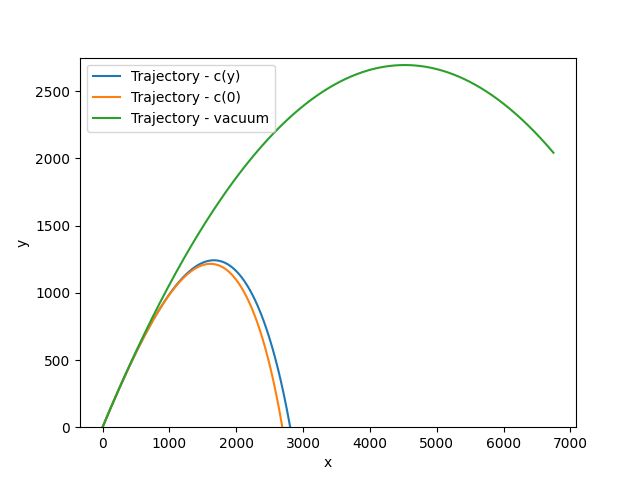
\includegraphics{taylor-2.44.png}
    \end{proof}
    \begin{proof}{\textbf{2.52}}
        We know that
        $$\eta = v_x + iv_y$$ but also 
        $$\eta = Ae^{-i\omega t} = ae^{i(\delta - \omega t)}$$
        then we can write $\eta$ as
        $$\eta = a\cos(\delta - \omega t) + ai \sin(\delta - \omega t)$$
        so making both expressions equal we get the values for each component
        $$v_x = a\cos(\delta - \omega t) \quad\quad v_y = a\sin(\delta - \omega t)$$
    \end{proof}

\end{document}






















